\begin{bclogo}[couleur = gray!20, arrondi = 0.2, logo=\bcattention]{Incremental code}
As for the last sessions, we provide you with a "golden version" of the project at this point. If you are not sure about the correctness of your implementation, download \texttt{p2d.patch} from Moodle and apply it to your repository. Note that the patches are incremental, meaning that you must apply \texttt{p2a.patch}, \texttt{p2b.patch} and \texttt{p2c.patch} (if not already done), then \texttt{p2d.patch} on top of it.
\end{bclogo}

\section{Measuring the instantaneous power consumption}

A common method to measure the instantaneous power consumption of a system is to use a \textbf{shunt resistor}, or current-sensing resistor, as in \autoref{fig:rshunt}. The current flowing through it is the same as the one flowing through the system of interest, it can be computed based on the voltage measured accross the resistor and its value. As the system supply voltage is fixed, you can simply multiply the instantaneous (or average) current by the voltage to get the instantaneous (or average) power consumption.

\subsection{MCU's consumption}
The Nucleo board provides an easy way of shunting the MCU, by removing the \textbf{JP5} jumper that cuts the supply and replacing it with the shunt resistor, as in \autoref{fig:jp5}.

The embedded system is supplied at \textbf{VDD = 3.3V} in its default configuration, check out the document \textit{Guide - How to use the boards} on Moodle for alternative configurations.

Use the second channel of the oscilloscope to \textbf{extract a power consumption trace} of the MCU during one acquisition-computation-transfer cycle, while the first channel is used as a trigger on GPOUT.

\begin{minipage}[b]{.45\textwidth}
	\begin{figure}[H]
	    \centering
	    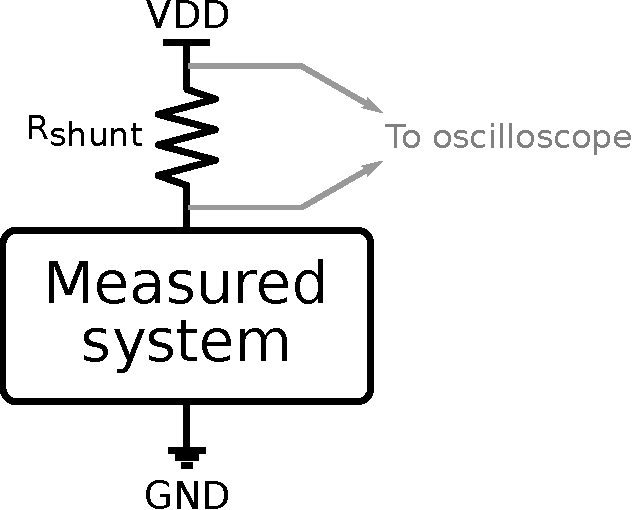
\includegraphics[width=.8\textwidth]{figures/rshunt.pdf}
	    \caption{Shunt resistor to measure the instantaneous power consumption.}
	    \label{fig:rshunt}
	\end{figure}
\end{minipage}
\hfill
\begin{minipage}[b]{.45\textwidth}
	\begin{figure}[H]
	    \centering
	    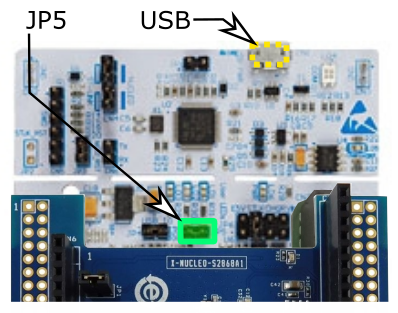
\includegraphics[width=.9\textwidth]{figures/JP5.png}
	    \caption{Remove JP5 and shunt the supply rail at this place.}
	    \label{fig:jp5}
	\end{figure}
\end{minipage}

\begin{bclogo}[couleur = gray!20, arrondi = 0.2, logo=\bcattention]{Choosing the right shunt resistor value}
The shunt resistor transduces current into voltage that you can then probe. Ideally, you'd want the measurement to be transparent regarding the operation of the system, i.e. no voltage drop at all. In practice however, the voltage you measure must be above the noise floor inherent to your measurement device. The ADALM being quite noisy, here is a good rule of thumb for clean and correct measurements :
\begin{itemize}
	\item $V_\text{shunt} > \SI{30}{\milli\volt}$ to obtain clean (non-noisy) traces ;
	\item $V_\text{shunt} < \SI{300}{\milli\volt}$ to limit the supply voltage pollution. Note that an exceedingly large voltage drop will make your device shutdown due to the protection mechanism (brown out reset) that triggers when VDD < 1.71V on your MCU.
\end{itemize}
\textit{Hint:} Use a multimeter in ammeter mode through JP5 to measure the average current consumption, then use this value to size your shunt resistor.
\end{bclogo}

\begin{bclogo}[couleur = gray!20, arrondi = 0.2, logo=\bcattention]{ADALM oscilloscope's systematic offset}
Each measurement device presents non-idealities that might bias the measurements if they are not negligeable. The ADALM oscilloscope has quite a high systematic offset (up to \SI{15}{\milli\volt} positive or negative) that you should substract from any measurement.

To measure your device's offset, simply tie the two probes of the channel together at the targetted common-mode voltage (the offset may be different at 0V and at 3.3V). For example, tie both \textbf{2-} and \textbf{2+} to \textbf{VDD} as it is the common-mode voltage at JP5. Write down the measured offset and substract it from any ulterior measurement.
\end{bclogo}

\begin{bclogo}[couleur = gray!20, arrondi = 0.2, logo=\bcinfo]{Data extraction for processing}
In Scopy, you can extract the data as a \texttt{csv} file. You may want to use this feature to compute the power consumption based on the shunt voltage and produce nice annotated plots.
\end{bclogo}

\begin{bclogo}[couleur = gray!20, arrondi = 0.2, logo=\bcquestion]{MCU power trace analysis}
Describe what you observe on the measured power consumption trace. Can you identify the phases of operation of your MCU (acquisition, computation, transfer) ? \textit{Hint:} Use GPOUT to help distinguish the tasks you want to identify.

Does you measurement correspond to what is expected when checking the power consumption indicated in the MCU's datasheet ?
\end{bclogo}

\subsection{Radio's consumption}

The radio board provides a similar way of cutting the supply rail to insert a shunt resistor. Locate \textbf{JP1 on the radio (blue) board} and use the same technique to measure the power consumption of the radio. Comment the measured power trace.

\subsection{AFE's consumption}

The analog frontend is the third and last subsystem that consumes electrical power. Locate \textbf{SUP-} and \textbf{SUP+} on the custom (green) board. These are two jumpers that cut the supply rail of the AFE. Measure its power consumption in operation and comment it.

\begin{bclogo}[couleur = gray!20, arrondi = 0.2, logo=\bcquestion]{Energy harvesting and power budget}
By summing the consumption of the three subsystems, you obtain the total power consumption of the embedded system. What is the average total power consumption during the active cycle ? How much time and how much energy does one cycle takes ?

In the future, you will harvest solar energy and supply your system by a solar cell. In nominal conditions, it will provide you with a power budget of around \SI{10}{\milli\watt}. Does your system fit in for now ? You should also take into account the efficiency of the power conversions made by the energy harvesting circuit.
\end{bclogo}

\section{Optimising the system's power consumption}

Herebelow are listed several ways of reducing the power consumption of the system. Note that the objective of this first semester is not to optimise your system at most, but rather to discover the leverages at your disposal and the tradeoffs that come with.

Describe the impact of each of the following parameter on the power consumption trace of the MCU and/or the radio. When relevant, do not hesitate to sweep a parameter among 3-5 values to describe its impact on the power consumption and identify its trend (linear or non-linear, saturation, etc).

\begin{itemize}
	\item{\textbf{Low-power mode}} Between two mel-vector computations, the CPU loops in active mode while not executing anything useful. Let it enter sleep mode by calling \texttt{\_\_WFI()} at the end of the main loop. It stands for \textit{wait for interrupt}, meaning that the CPU will wake up whenever an interrupt arises.
	\item{\textbf{LED}} Stop lighting on the blue LED when performing the acquisition. How much power does the LED consume ?
	\item{\textbf{CPU clock frequency}} In STM32CubeMX, go to the \textbf{Clock Configuration} tab. On the left, reduce the \textbf{MSI RC} oscillator frequency down to \textbf{24MHz}. This generates the clock feeding the CPU, but also the timers. Don't forget to update the prescaler of the timer 3 to keep acquiring at \SI{10}{\kilo\hertz}. What is(are) the main constraint(s) associated with it ?
	\item{\textbf{Radio output power}} Change the emission power of the radio by setting the value of \texttt{PA\_LEVEL} in \texttt{config.h}. It can be set between \SI{-30}{\dBm} and \SI{14}{\dBm} (cfr. its datasheet).
	\item{\textbf{Feature vector length}} Modify the number of mel-vectors per feature vector \texttt{N\_MELVECS} in \texttt{config.h}.
\end{itemize}
